Nous avons implémenté deux extensions supplémentaires qui apportent des fonctionnalités supplémentaires mais aussi de la compléxité au système. C'est pourquoi nous avons les avons implémenté en parallèle et façon à ce qu'elles soient indépendantes entre elles.

\section{Gestion plus fine des ressources}

\subsection{Transformation SimplePDL vers PetriNet}

\section{Ressources alternatives}

Il s'agit ici de mettre en oeuvre une gestion alternative des ressources. Le principe est qu'il existe plusieurs configurations possibles de ressources.
Ainsi, soit une configuration A nécéssitant 2 machines et 3 développeurs et une configuration B avec 3 machines et 2 testeurs, on pourra exprimer le fait qu'une WorkDefition a besoin que la configuration A ou que la configuration B soit effective.

\subsection{Redéfinition du méta-modèle}

Il est donc clair que l'on doit modifier le méta-modèle pour expliciter cette possibilité de ``regroupement des ressources''.

\begin{figure}[!h] 
\begin{center}
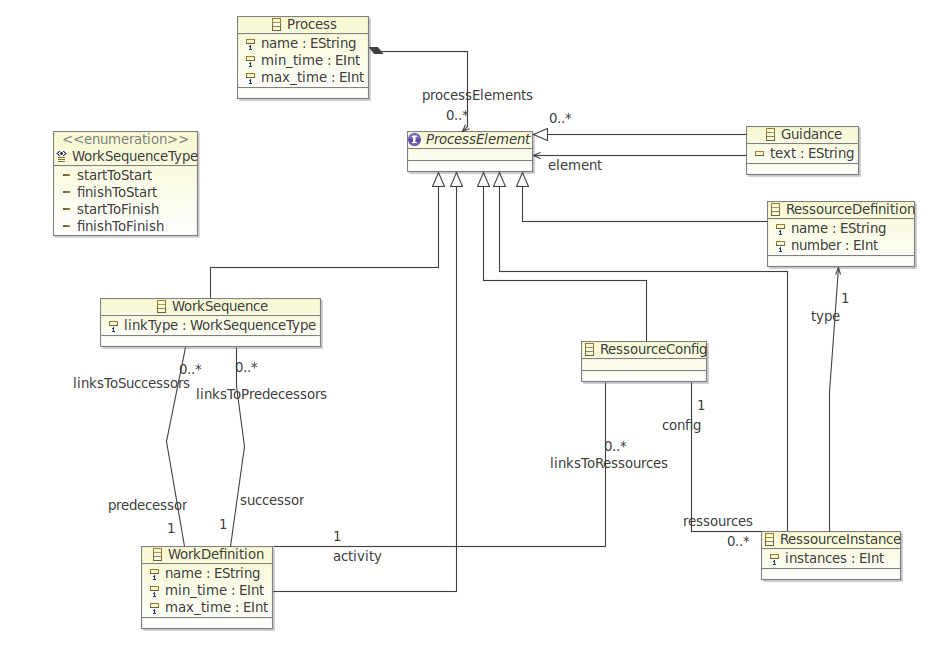
\includegraphics[width=15cm]{Capture-13.png}
\caption{Méta-modèle avec ressources alternatives} 
\label{img1} 
\end{center}
\end{figure} 

Et sous forme graphique,\\

\newpage

\begin{figure}[!h] 
\begin{center}
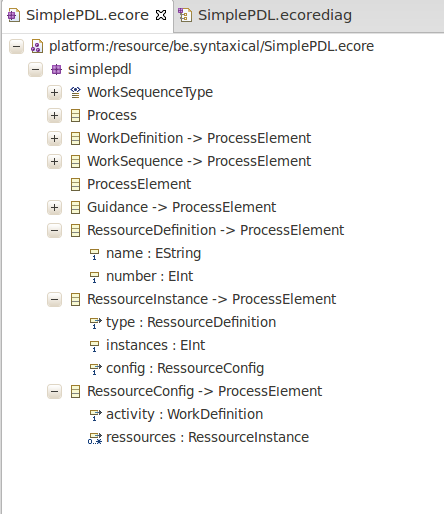
\includegraphics[width=8cm]{Capture-14.png}
\caption{Méta-modèle sous forme graphique} 
\label{img1} 
\end{center}
\end{figure} 

Pour permettre ce regroupement, on rajoute une classe RessourceConfig. Cette classe va contenir des liens vers des RessourceInstance. Ainsi, on va exprimer le fait qu'il peut exister plusieurs configurations mettant en oeuvre différents jeux de ressources.\\

On remplace donc le lien de WorkDefinition a RessourceInstance, par un lien de WorkDefinition a RessourceConfig. Ce lien a une multiplicité 0..\* car on peut avoir plusieurs Configurations pour une même WorkDefinition.

\subsection{Transformation SimplePDL vers PetriNet}

Prenons l'exemple suivant, 

\begin{figure}[!h] 
\begin{center}
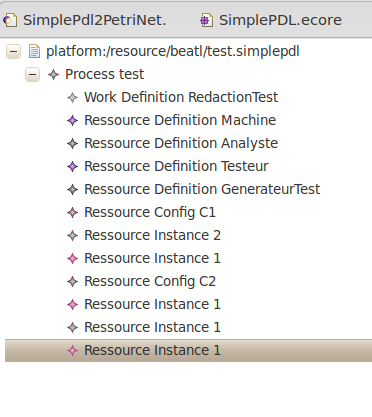
\includegraphics[width=8cm]{Capture-15.png}
\caption{Exemple mis en oeuvre} 
\label{img1} 
\end{center}
\end{figure}

On dispose de 4 ressources : Machine, Analyste, Testeur, GenerateurTest.
Par souci de lisibilité, on limite le nombre de WorkDefinition, à une seule : redactionTest. On définit également deux configurations C1 et C2. C1 met en oeuvre deux WorkInstance (Machine, 2) et (GenerateurTest,1). C2 met en oeuvre trois WorkInstance (Analyste,1), (GenerateurTest,1) et (Machine,1).\\

Cet exemple va nous permettre d'illustrer les transformations qui doivent être effectuées.\\

Il faut donc reprendre la transformation SimplePDL vers PetriNet et transformer la gestion des Ressources. Toujours par souci de lisibilité, on s'affranchit de la génération d'observateurs.\\

Le principe du réseau de pétri gérant la configuration des ressources est le suivant :\\

\begin{itemize}
\item Il est possible de choisir entre chacune des configurations (si du moins il y a suffisament de ressources)
\item Une fois que l'on a choisi de démarrer avec une configuratio, on ne pourra plus choisir l'autre
\item Les Ressources utilisées doivent être restituées à la fin de l'activité, et qui plus est dans la bonne configuration.
\end{itemize}

Il ressort de cette analyse que l'on va devoir utiliser des places nous indiquant :\\

\begin{itemize}
\item Quelle configuration est choisie : ConfigurationName\_used
\item Une configuration a été choisie : ProcessName\_ress\_l\\
\end{itemize}

Et des transitions pour :\\

\begin{itemize}
\item Choisir une configuration : ConfigurationName.start
\item Rendre les ressources : ConfigurationName.finished\\
\end{itemize}

Pour l'exemple cité précédement, on obtient donc le réseau de pétri suivant :\\

\begin{figure}[!h] 
\begin{center}
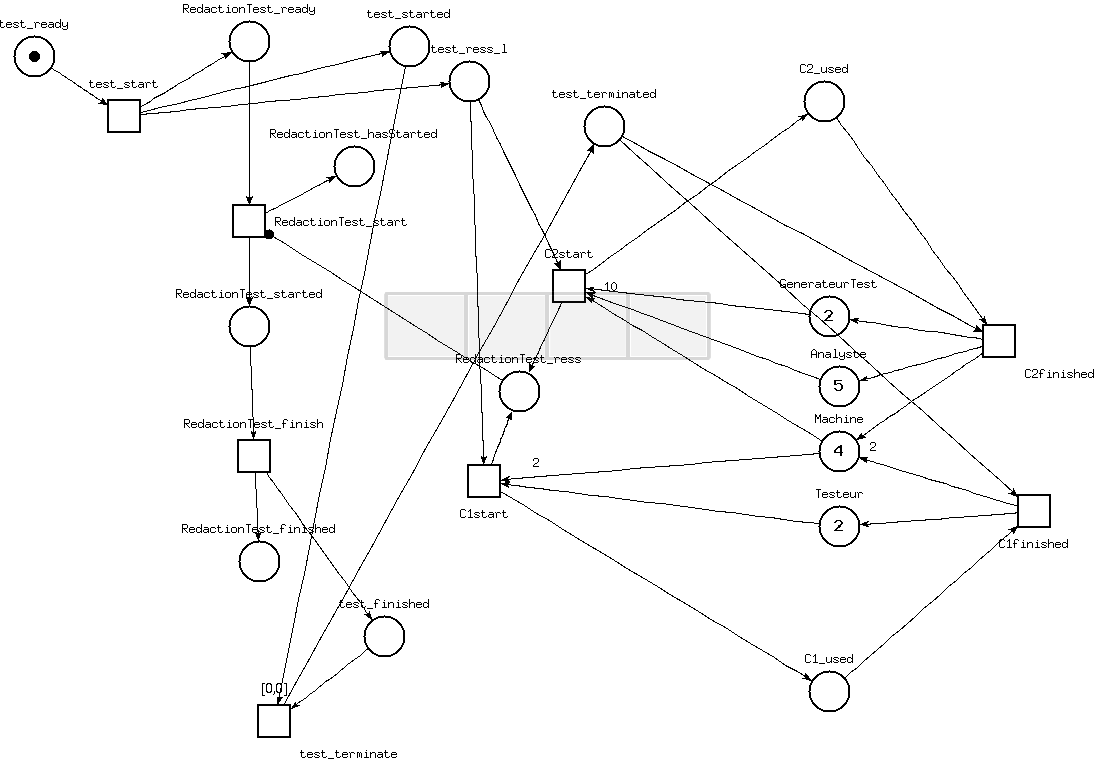
\includegraphics[width=15cm]{Capture-16.png}
\caption{Réseau de pétri obtenu} 
\label{img1} 
\end{center}
\end{figure}

Bien entendu, le code de la transformation a été adapté pour fornir ces changements. Il est disponible en annexe.\\

Pour ce qui est de la transformation PetriNet2Tina, il n'y a toujours aucune raison de la modifier car, on a pu conserver la même structure pour le méta-modèle PetriNet.ecore.\\







